\documentclass[paper]{ijdc-v9}
\usepackage[T1]{fontenc}
\usepackage{lmodern}
\usepackage{amssymb,amsmath}
\usepackage{ifxetex,ifluatex}
\usepackage{fixltx2e} % provides \textsubscript
\usepackage{booktabs}
\usepackage{dcolumn}
\usepackage{longtable}

\usepackage{biblatex}
\bibliography{}

\providecommand{\tightlist}{%
  \setlength{\itemsep}{0pt}\setlength{\parskip}{0pt}}


\title[Agile Data Curation]{Agile Data Curation as a Diversity of Practices Grounded in Shared
Values and Principles}


\author{Karl Benedict}
\affil{University of New Mexico}
\author{W. Christopher Lenhardt}
\affil{Renaissance Computing Institute}
\author{Joshua Young}
\affil{University Corporation for Atmospheric Research}

\correspondence{Karl Benedict, MSC05 3020, 1 University of New Mexico, Albuquerque, NM 87131. Email: \email{kbene@unm.edu}}


\begin{document}
\maketitle

\begin{abstract}
Current research data management and curation practices can be described
as falling along a continuum between highly engineered systems and
ad-hoc practices or nothing at all. In recognition of the increasing
investment in and importance of research data as an asset for doing
research, for evaluating current research results, and as a resource for
new science, funding agencies, publishers and some research teams have
instituted research data management practices. These practices are often
aligned with a wide variety of data life cycle models that embody a
circular process of activities that include creation, assessment,
documentation, use, preservation, discovery and reuse. While these data
lifecycle approaches are well aligned with the documentation and
preservation of research data - particularly as they have been primarily
developed by organizations with a mandate to provide for the
preservation of data, this linear (or more appropriately cyclical) model
does not necessarily focus on the level of effort required throughout
the processes embodied in the lifecycle or the lowering of barriers to
subsequent reuse. The agile data curation conceptual model outlined
provides is proposed as a starting point for community consideration a
core set of values, principles and in the long-run recommended practices
in the form of research data management and {[}agile{]} curation design
patterns that may be used to define project-specific activities that are
likely to both meet the immediate needs of data producing research
projects while also maximizing the net value of data produced by those
projects for future research, education, and applications. \emph{{[}This
last sentence is the crux of the argument/paper. I think though we left
out a step. That is the design patterns support agile curation which
reduces burden, yadda, yadda, which then supports projects and maximizes
value. I added for consideration the word {[}agile{]} before curation
design patterns which address this in part. However, does this need
more? Also, I could figure out how to put this in as a comment, so I
inserted it this way.{]}}
\end{abstract}

\section{Overview}\label{overview}

The challenges that must be addressed by current research data
management and curation processes and strategies consist of a
combination of established practices that are not compatible with
increasing complexity in the data management landscape at the project
level; increasing expectations by sponsors, publishers, and institutions
relating to data management and curation; and rapid growth in the
volume, variety and velocity (three dimensions commonly used to define
``big data'') of data generated by and used in research. In combination
these challenges translate into an increasing need to develop effective
data management and curation strategies that align with a set of shared
values and principles that inform management and curation objectives,
and implement processes that are well documented and portable across
specific data management projects.

The concept of \emph{agile data curation} outlined in this paper
represents an effort by the authors to develop a conceptual model for
data management and curation that extends beyond the linear or cyclical
model represented by the many data lifecycle models that have been
developed
\autocites{ball_review_2012}{park_session_2016}{moller_lifecycle_2013}{working_group_on_information_systems_and_services_data_data_stewardship_interest_group_data_2011}.
These lifecycle models have been created to define processes that are
more structured than the commonly used ad-hoc or minimally designed
research processes that are not explicitly developed to meet the full
arc of activities that meet the needs of both the current research
activity \emph{and} those of future users of the data products generated
by that activity
\autocites{kervin_common_2013}{white_considering_2010}{tenopir_data_2011}{akers_disciplinary_2013}{kennan_research_2015}{vines_availability_2014}.

In response to this problem of under-design and with the increasing
recognition of the value of research data products for assessment,
replication, validation, and extension of research, a variety of
requirements have been put in place by sponsors
\autocites{office_of_management_and_budget_omb_digital_2012}{office_of_management_and_budget_omb_memorandum_2013}{office_of_management_and_budget_omb_memorandum_2009}{obama_77_2012}{obama_executive_2013}{obama_transparency_2009}
and publishers \autocites{_availability_2016}[
]{public_library_of_science_plos_data_2016} for planning for and
executing effective data management, sharing, and curation. While these
requirements have resulted in more explicit documentation of
\emph{plans} for data curation and management, it remains unclear what
impact they are having on \emph{practice}.

{[}Do we want to have a paragraph here from the data creator
perspective? That is the widely held perspective that doing curation
work is onerous and gets in the way of doing science, etc. Are there any
cites we can dig up on this? One that comes to mind is the data entropy
one from Bill M.{]}

While the increasing requirements for planning and execution of
systematic data management and curation have resulted in additional
attention to these topics, there has not been a corresponding increase
in funding in support of these activities. The challenge of fitting
these required management and curation activities within existing funds
is compounded by the continuing (often characterized as exponential)
growth
\autocites{turner_executive_2016}{national_aeronautics_and_space_administration_nasa_heasarc_2016}
in created, managed and requested data within those limited resources.
These increasing demands within a consistently resource constrained
environment increase the value of developing data management and
curation objectives and strategies that are likely to maximize the
current and future value of research data within available resources.

Given this context, the authors have (with contributions from
participants in workshops and meeting sessions held over the past two
years in multiple venues) been considering the agile software
development movement \autocite{beck_manifesto_2001} as a source of
inspiration for the development of a conceptual model for \emph{agile
data curation} that balances the needs for robust documentation and
engineered solutions with a development cycle that is designed for
incremental delivery of value through an iterative development and
investment process. From the discussions held with researchers and data
managers participating in meetings of the Federation of Earth Science
Information Partners (ESIP), American Geophysical Union (AGU), the
Research Data Alliance (RDA), and SciDataCon the authors have had an
opportunity to explore and refine some of the key concepts relating to
agile data curation as it is both similar and dissimilar from agile
software development.

Figure 1 illustrates a number of the shared and different
characteristics that have been identified that may be ascribed to the
ends of the continuum between highly designed/engineered processes and
ad-hoc processes in both software development and data curation. A
common theme that has emerged in the discussions around this topic over
the past two years has been that while the agile software development
movement partially emerged in response to the observed shortcomings in
the commonly employed, specification heavy, and long development cycle
``waterfall'' development model, the proposed agile data curation model
is largely a response to ad-hoc data management practices that are
frequently the norm for research projects - particularly small research
projects for which there are not dedicated data management and curation
resources, dark data in Heidorn's \autocite*{heidorn_shedding_2008}
terminology. While there are exemplars of highly successful software
development and data curation practices at all points along the
continuum illustrated in Figure 1, the adoption of agile software
development practices in the middle range of the continuum has allowed
some projects to achieve success where they may have otherwise been
unsuccessful, and likewise data curation activities that have
successfully moved from the right end of the continuum towards the
center have also provided measurable value to both the current projects
that are creating the data and to future users of the data produced by
those projects. It is these successful data curation projects that
exemplify an emerging set of values, principles and practices of agile
data curation that provide the foundation for the design pattern
activity of the research team that is described below.

\begin{figure}[htbp]
\centering
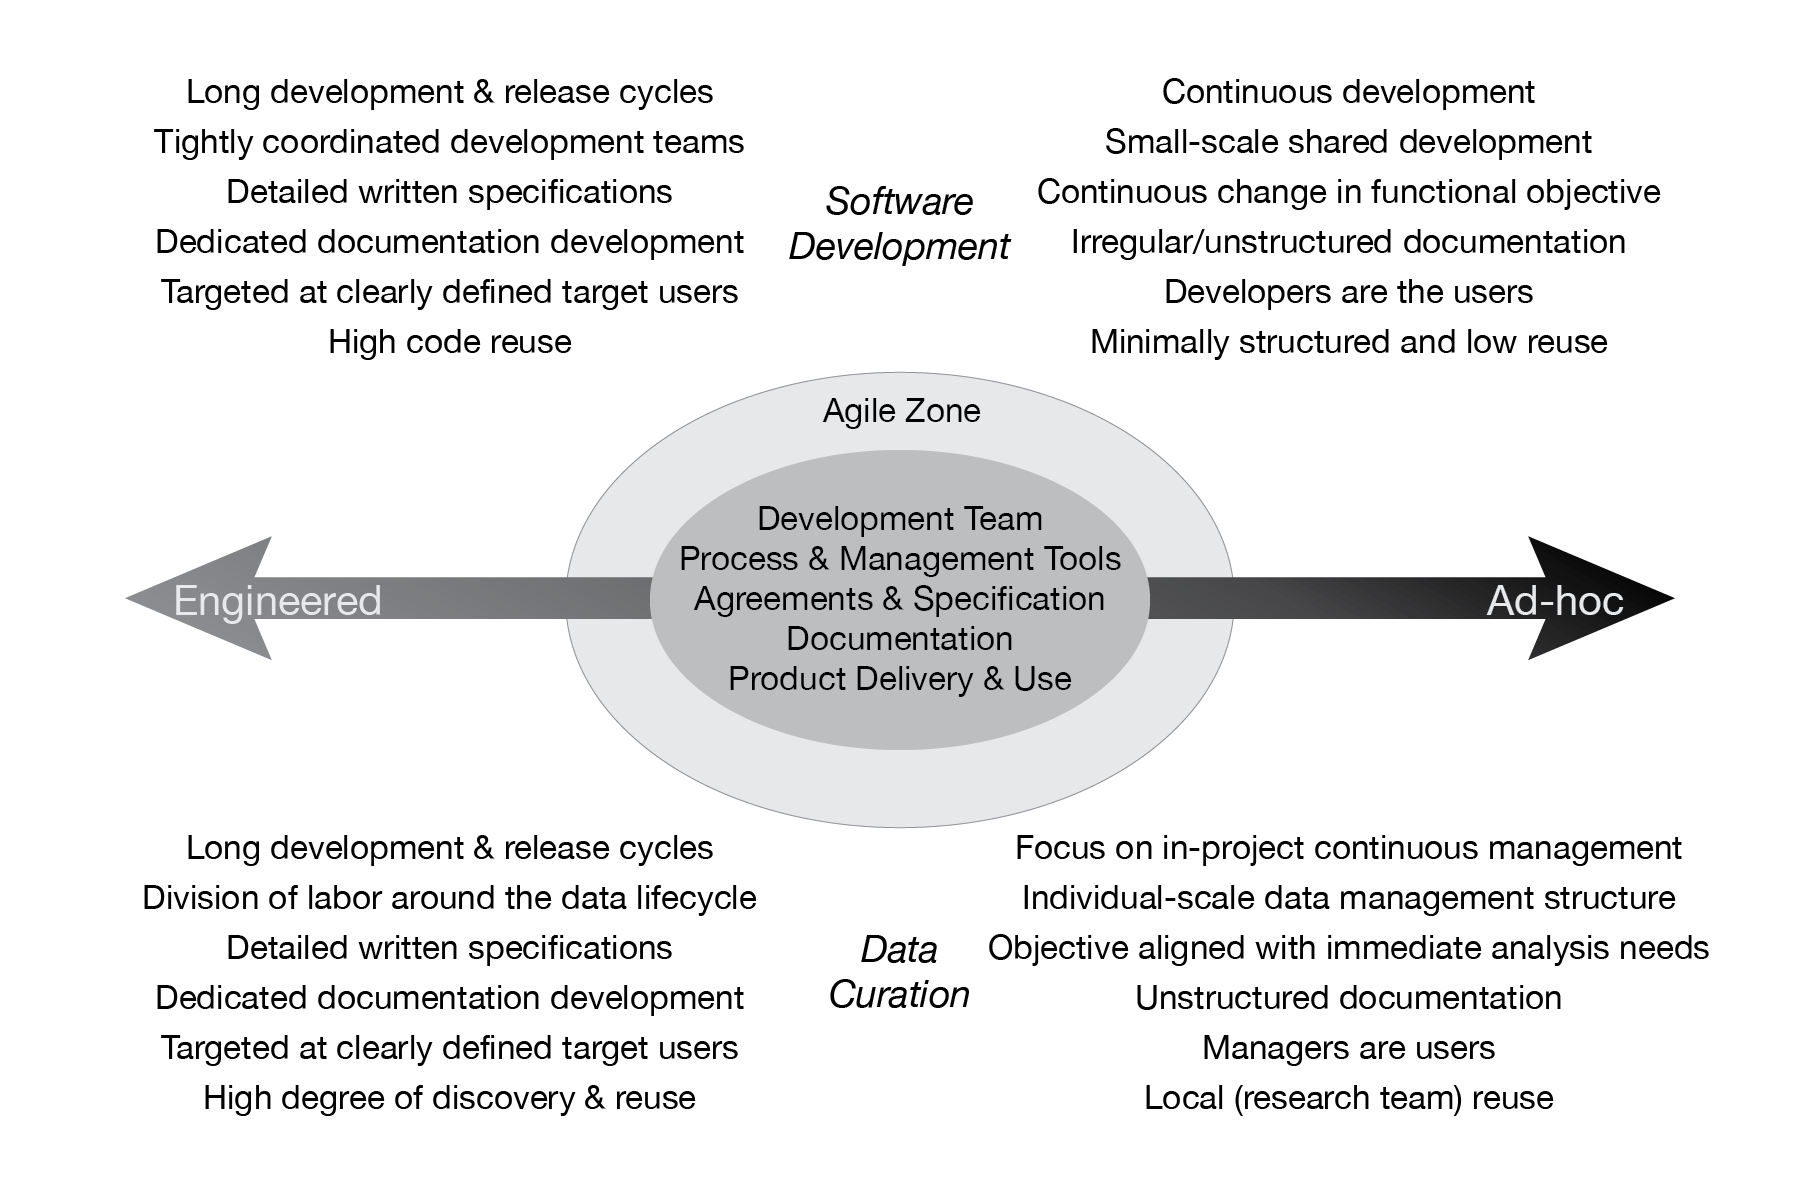
\includegraphics[width=5.00000in]{agileComparison-01.png}
\caption{Illustration comparing software development and data curation
activities along a continuum between \emph{engineered} and \emph{ad-hoc}
highlighting a range of characteristics associated with with each
activity, and the mid-point along the continuum where an agile approach
can hopefully achieve a balance between the two extremes.}
\end{figure}

====== begin notes ======

Following the model developed by the agile software development
communityThe set of values and principles developed by members of the
software development community around the concept of \emph{agile
software development} provides a potential framework from which a set of
agile data curation and management values and principles can be derived.
Once a set of values and principles have been developed the community of
research data producers and consumers is in a position to develop and
use practices that are informed by those principles.

The objective of this paper is to propose\footnote{link to a web site
  where community input can be collected and collated into something
  like the \emph{Manifesto}} a set of \emph{agile data curation} values
and principles that parallel those developed by members of the software
development community, but reflect the distinctive characteristics and
challenges posed by the research data process and its products.

\begin{itemize}
\tightlist
\item
  Continuum from ``Engineered'' \textless{}==\textgreater{} ``Agile''
  \textless{}==\textgreater{} ``Ad-hoc'' (Josh)

  \begin{itemize}
  \tightlist
  \item
    Technical debt as another dimension for characterizing

    \begin{itemize}
    \tightlist
    \item
      Model technical debt as increasing cost/reuse value as time passes
    \item
      Data entropy as a dimension (increased investment in metadata,
      data structure, preservation can reduce the slope for the entropy
      curve)
    \end{itemize}
  \item
    Dimensions to think about:

    \begin{itemize}
    \tightlist
    \item
      Required Formats
    \item
      Required data schemas
    \item
      Required file nameing conventions schemas
    \item
      Required metadata/documentation content
    \item
      Required metadata standards
    \item
      Approvals required
    \end{itemize}
  \end{itemize}
\item
  Recognize cost of capture/creation, management, sharing and
  preservation and build prioritization into decision making about what
  products/parameters are maintained within the system.
\end{itemize}

\section{Methods (1000)}\label{methods-1000}

** note: Justification of use of agile principles for activities outside
of software engineering**

For the development of the design patterns we have a three-part
approach. First we are comparing and contrasting the current generally
accepted/representative models which guide data curation with the key
concepts of agile development. The goal is to see how easily the zen of
agile software can map to data curation in the abstract.

Our second activity is to gather case study data that illustrate extant
practices that reasonably fit the ethos (read conceptual framework) of
agile curation. Cases are self-selected at this point by the submitter
as an example of an agile curation process. {[}Do we want to include an
example of a case?{]}

** note: design patterns as an alternative conceptual model for ``best
practices'' {[}granular{]} and/or lifecycle {[}abstract{]} approaches**

\section{Discussion}\label{discussion}

\begin{enumerate}
\def\labelenumi{\arabic{enumi}.}
\item
  Concept mapping (Josh - 800-1000) - have done this, capture here. Talk
  about vetting of this so far by community. i.e.~the papers / posters /
  sessions we've had to date. What have we learned. What are the areas
  of push-back?
\item
  Case studies (Chris - 800-1000) - in process, developed tool to
  capture examples.
\item
  Proposed design pattern process (Karl - 800-1000) -
\end{enumerate}

The application of the concept of agile data curation design patterns is
based upon the concept initially developed for object oriented software
development \autocite{gamma_design_1995}, and extended into related
domains
\autocites{daigneau_service_2011}{lasater_design_2010}{ackerman_patterns-based_2010}{schwinn_design_2005}{hohpe_enterprise_2003},
for use in documenting common \emph{named} data curation
\emph{problems}, \emph{solutions}, and \emph{consequences} that provide
\emph{descriptions of generalized data components that are customized to
solve a general design problem in a particular context} (adapted from
\autocite[section 1.1]{gamma_design_1995}).

The conceptual model that the research team has developed for mapping
research data curation functional requirements into design patterns
represents a combination of specific research activities that have
data-related components (as exemplified in Figure 1) and linkages
between those components as envisioned by a model such as the \emph{Open
Archival Information System} (OAIS -
\autocites{book_reference_2012}{_iso_2012}{oclc_open_2014} - Figure 2).
In particular, the research team is currently developing a model for
collecting and synthesizing data curation case studies that can be used
as exemplars for identifying existing design patterns or developing new
ones that are relevant in data curation.

\begin{figure}[htbp]
\centering
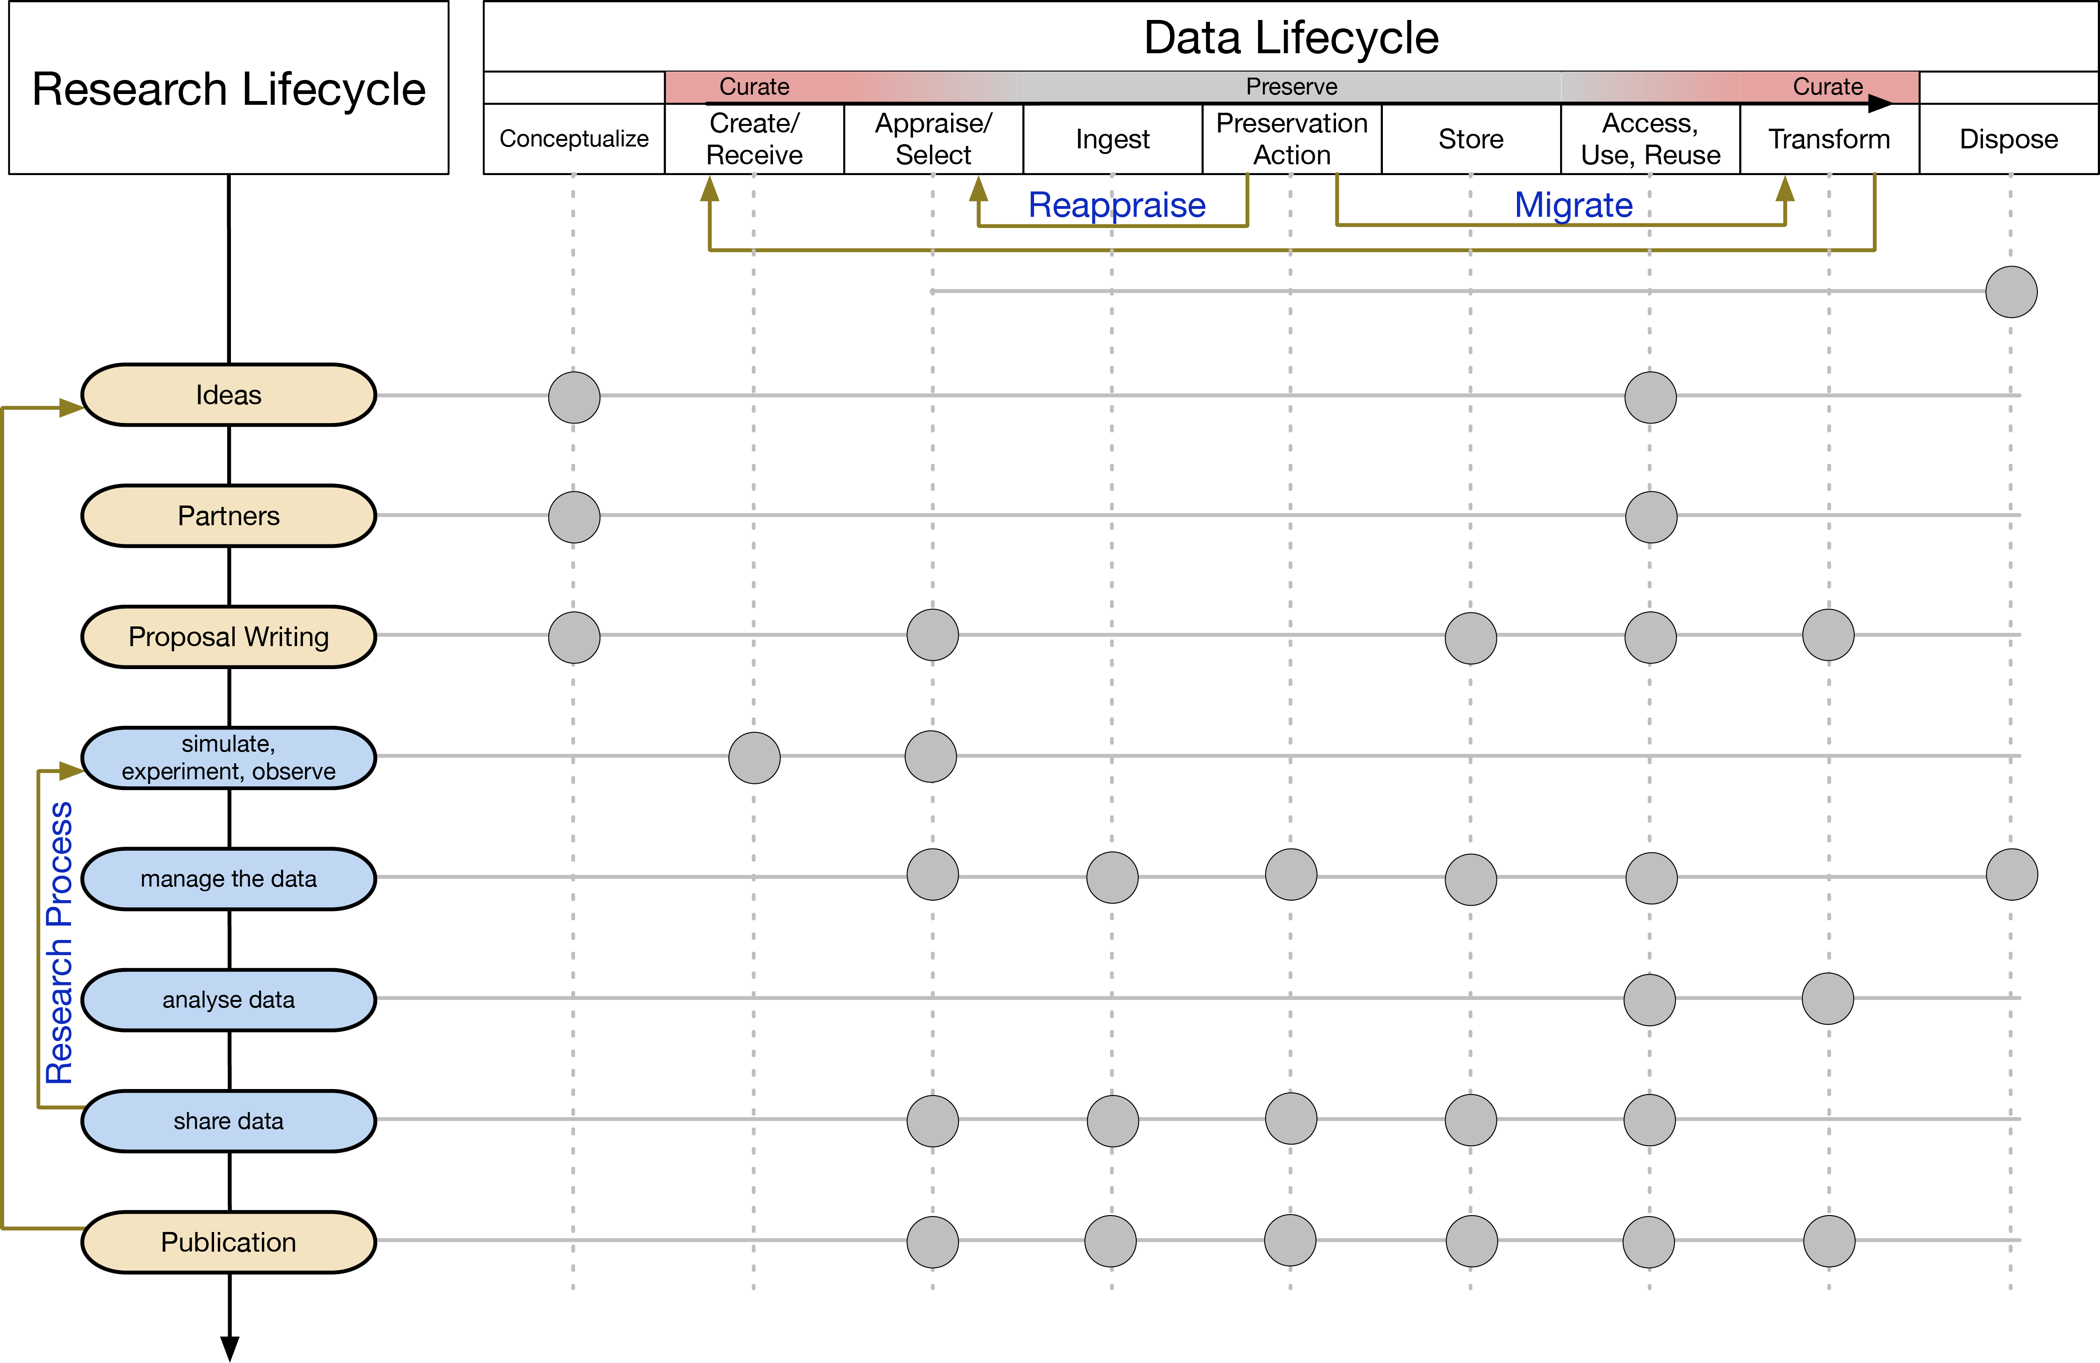
\includegraphics[width=5.00000in]{Research-DataLifecycleIntegration.png}
\caption{Intersection of Research Lifecycle \autocite{_how_2014} and
Data Curation Lifecycle Actions
\autocite{digital_curation_centre_dcc_dcc_nd} illustrating high-level
research activities that involve data-related functions.}
\end{figure}

The process that the research team proposed in support of the
identification and, when needed, development of agile data curation
design patterns consists of the following steps:

\begin{enumerate}
\def\labelenumi{\arabic{enumi}.}
\tightlist
\item
  Reach out to the research data curation community to seek specific
  research data problems for which effective solutions have been
  developed. {[}Note: add concept of \emph{anti-patterns} using
  references from https://en.wikipedia.org/wiki/Anti-pattern as an entry
  point{]}
\item
  From this compilation of case studies begin the development of a
  catalog of \emph{common} problems and solutions from which candidate
  patterns can be identified
\item
  Compile a catalog of existing design patterns against which the
  identified problems and solutions can be compared to identify
  opportunities for reuse of existing design patterns
\item
  Develop RFC design pattern proposals for review and comment by the
  research data management community (e.g.~RDA, ESIP Federation, IDCC
  participants, \ldots{})
\item
  Integrate feedback on proposed design patterns into final versions for
  publication.
\end{enumerate}

\section{Conclusions}\label{conclusions}

These are our conclusions

\section{Acknowledgements}\label{acknowledgements}

This would not have been possible without \ldots{}

\end{document}
